% \documentclass[12pt]{ociamthesis}  % default square logo 
\documentclass[12pt,beltcrest]{ociamthesis} % use old belt crest logo
% \documentclass[12pt,shieldcrest]{ociamthesis} % use older shield crest logo

%load any additional packages
\usepackage{enumerate}
\usepackage{amssymb}

\usepackage{amsmath}
\usepackage{bbm}
% \usepackage[round]{natbib}
\usepackage{varioref}
\usepackage{algorithm}
\usepackage{algpseudocode}

\usepackage{amsthm}
% \usepackage{natbib}
\usepackage{apalike}
% \usepackage{todonotes}

\usepackage{pdfpages}


%input macros (i.e. write your own macros file called mymacros.tex 
%and uncomment the next line)
\newcommand{\R}{{\mathbb R}}
\newcommand{\C}{{\mathbb C}}



% \newcommand{\poly}{{\mathbb R}}
\newcommand{\poly}[2]{Li_{#1} ({#2})}
\def\mean#1{\left< #1 \right>}

% \def\ramp{\rho^*}
\def\ramp{\rho}
% \def\rmat{\hat{\rho}}
\def\rmat{C}
% \def\rij{\rho_{ij}}
\def\rij{c_{ij}}
\def\rji{c_{ji}}
\def\rii{c_{ii}}

 
\theoremstyle{definition}
\newtheorem{definition}{Definition}[section]
 
\theoremstyle{lemma}
\newtheorem{lemma}{Lemma}[section]


\theoremstyle{remark}
\newtheorem*{remark}{Remark}

\newenvironment{proof}{\paragraph{Proof:}}{\hfill$\square$}

\theoremstyle{theorem}
\newtheorem{theorem}{Theorem}[section]


\title{Network modelling
of credit concentration risk}
%note \\[1ex] is a line break in the title

\author{Candidate Number 187489}        %your name
\college{Kellogg College}  %your college

%\renewcommand{\submittedtext}{change the default text here if needed}
\degree{MSc in Mathematical Finance}     %the degree
\degreedate{Trinity 2016}         %the degree date

%end the preamble and start the document
\begin{document}

%this baselineskip gives sufficient line spacing for an examiner to easily
%markup the thesis with comments
\baselineskip=18pt plus1pt

%set the number of sectioning levels that get number and appear in the contents
\setcounter{secnumdepth}{3}
\setcounter{tocdepth}{3}


\maketitle                  % create a title page from the preamble info
\chapter*{Acknowledgements} % (fold)
\label{cha:acknowledgements}


I would like to thank my supervisor Dr. Peter Gl\"ossner for the suggestion of the topic, for his guidance, for the valuable comments and for the open and inspiring discussion rounds that lead to this thesis.

I extend my sincere thanks to Dr. Michael Monoyios, University of Oxford, who was always very cooperative - both in scientific and administrative issues.

Several colleagues at d-fine GmbH gave me useful hints in the progress of preparing this thesis.
In particular I would like to thank Dr. Anne Kleppe, who provided insight and data, and Dr. Walter Freyn, who provided helpful feedback.

I am much obliged to d-fine GmbH for supporting my studies at the University of Oxford in the part time Mathematical Finance program.

Finally, I would like to thank my family, Anne and Leo, for putting up with me during my studies at Oxford. Merci!


% chapter acknowledgements (end)        % include a dedication.tex file
% \chapter*{Authenticity Statement} % (fold)
\label{cha:authenticity_statement}

I hereby declare that this thesis is my own work and confirm its authenticity.

\vspace{1cm}
\begin{tabular}{l l}

\textbf{Name:} & Miguel Vaz\\
\\
\textbf{Address}: & Wittelsbacherallee 151\\
& 60385 Frankfurt am Main\\
& Germany\\
\\
\textbf{Signed:}& \\
\\
\\
\textbf{Date:}& December 16, 2016\\
\end{tabular}

% chapter authenticity_statement (end)      % include an acknowledgements.tex file
\begin{abstract}
plenty of waffle, plenty of waffle, plenty of waffle, plenty of waffle,
plenty of waffle, plenty of waffle, plenty of waffle, plenty of waffle.
\end{abstract}
          % include the abstract

\begin{romanpages}          % start roman page numbering
\tableofcontents            % generate and include a table of contents
\chapter*{Notation} % (fold)
\label{cha:notation}

Following notation will be used throughout this document:
\begin{itemize}
	\item[$k$] the degree of a vertex
	\item[$c$] the mean degree of a graph
	\item[$\mean{k}$] the average degree of a graph
	\item[$p_k$] the probability that a randomly chosen vertex has degree $k$
	\item[S] the fraction of vertices that belong to the giant component of a graph
	\item[u] the fraction of vertices that do not belong to the giant component of a graph
\end{itemize}
% chapter notation (end)Notation:
          % include the abstract
\listoffigures              % generate and include a list of figures
\end{romanpages}            % end roman page numbering

%now include the files of latex for each of the chapters etc
\chapter{Introduction}



Banking regulators (Basel II) require market participants to identify and monitor concentration risk in their credit portfolios.
Concentration risk is the risk arising from high exposure to single risk factors.
Standard concentration measures rely mainly on the aggregation of the measures of each portfolio element at, for example, the economic sector of activity~\cite{lutkebohmert2008concentration}.
While these models performs well at predefined aggregation levels, they usually underestimate direct obligor-specific economic links and, possibly, the latent dependency structure of the portfolio.
The importance of structural measures has been confirmed by recent financial events, where large losses arising from worldwide contagion effects were registered~\cite{Kazi:2013vr}.
	
Network models are especially apt at identifying structural properties~\cite{newman2010networks}, as they take not only model the elements of a system (the nodes or vertices) but also the relations between those elements (the edges).
Network models are proving to be useful tools for providing early-warning signals of systemic risk~\cite{Squartini:2013ev}, measuring liquidity risk~\cite{Karas:2012tp}, identifying sectors from time-series correlations~\cite{Onnela:2004vz,Fenn:2009uf,Fenn:2011kp}, as well as insights into finding diversified baskets of assets in the classical investment framework~\cite{Pozzi:2013ci}.
Many other use cases are described in the recent book~\cite{Soramaki2016}.

Previous work on concentration risk relied on a network intepretation of a portfolio~\cite{Sindel:2009vd} by using a varying (ramping) parameter for progressively eliminating interdependencies between obligors, and analysed the relative exposure size of the component with largest exposure.
Using a weight function, this relative exposure size is integrated over all parameter values in order to measure the portfolio's concentration risk.

While this method is able to measure properties of specific portfolios, little is hitherto know about the expected properties of the model for a given portfolios.
% The expected properties could prove helpful to help identify idiosyncrasies of the model's behaviour on the specific portfolio at hand.
The main goal of this thesis is to connect ramping parameter model with theoretical work behind random graphs.
For this, we study the properties of the ramping parameter under the most widely theoretical graph model: the random graph model described by~\cite{erdos1959random}.
Firstly, having the model inspected theoretically allows for a better understanding of its properties.
Secondly, even though the theoretical models do not capture all the properties of real world graphs, it provides useful baselines for comparison with the results with real portfolios.


% The main goal of this thesis is to address the computational complexity of the method by providing a link to other common structural graph measures, e.g. eigenvector centrality, and financial specific measures, such as Debt-Rank~\citep{Puliga:2012ev} which models contagion effects from interdependencies of financial institutions.
% In order to do so, we will first study the properties of different theoretical network formation models (e.g. Watts–Strogatz model~\citep{Watts:1998db}.
% In a second stage, real credit portfolios will be used. Should time permit, the effect of different types of interdependencies will be studied by means of multilayer networks~\citep{Kivela:2014dm}.



\section{Credit concentration risk} % (fold)
\label{sec:credit_concentration_risk}

Under Basel II~\cite{basel2007explanatory}, banks are required to compute the capital requirements for their credit portfolios using the ASFR (Asymptotic Single Risk Factor)~\cite{}, and are allowed to use their own internal risk measurements - IRB approach.
The ASRF model is based on the results from~\cite{vasicek1991limiting} depends on three main quantities:
\begin{itemize}
	\item[PD] the Probability of Default: the probability that a considered obligor will default within the next 12 months,
	\item[LGD] Loss Given Default: the expected fractional loss in case of the obligor's default,
	\item[EAD] Exposure At Default: the expected exposure an obligor has when the default event occurs as seen from today.
\end{itemize}
While we urge the reader to refer to~\cite{Sindel:2009vd} for a more comprehensive description of the meaning of the quantities and how these are combined in the model, it is important to state that the ASRF model makes two important assumptions on the portfolios: 
\begin{enumerate}
	\item they are perfectly fine grained, thereby containing no idiosyncratic risk, i.e. no Concentration Risk
	\item there is only one source of systematic risk.
\end{enumerate}
In order to circumvent this limitation, the concentration risk, i.e. the probability of losses arising from an outstanding credit exposure to a given set of counterparties through some common risk factors, is accounted for by the so-called granularity adjustment (GA)~\cite{lutkebohmert2008concentration}.

We outline the different strategies behind the existing methodologies for assessing the Concentration Risk
\begin{itemize}
	\item concentration of absolute exposure, e.g. by means of the HHI (Herfindahl-Hischmann Index)
	\item a measurement of relative exposure concentrations, e.g. by using the Lorenz-Curve
	\item comparison with a given benchmark portfolio
\end{itemize}
As can be seen, the first two measures here rely solely on the exposure structure of the portfolio.
The measure proposed by~\cite{Sindel:2009vd} goes beyond this by relying on both the exposure- and the correlation-structure of the portfolio.

% section credit_concentration_risk (end)

\section{The ramping parameter model} % (fold)
\label{sec:ramping_parameter}

The ramping parameter model was developed in~\cite{Sindel:2009vd} and aims at assessing the concentration risk in real world loan portfolios. 
In contrast to other methods for studying concentration risk, the ramping parameter takes into account both, the exposure- and the dependency-structure of the portfolio.
A particular strength of this methodology is that it can be used universally.
% Through the course of this thesis, the 

The ramping parameter monitors how the component structure - notably the component with largest exposure - of a graph representing the considered portfolio develops, as edges are removed increasingly according to their strength.
% It computes a curve that parameterizes the dependency of the effective exposure on the ramping parameter.
We begin by defining some quantitites.

\begin{definition}{Portfolio}
A credit portfolio is a tuple $(O, \rmat)$, where $O$ is a set of $n$ exposures from $n$ different obligors and $C$ an $n \times n$ matrix.
The $\rmat$ matrix represents the interdependency (or correlation) between each obligors $i$ and $j$, and each element $\rij \in [0,1]$.
\end{definition}

\begin{remark}
Throughout this work, the matrix $\rmat$ is symmetric, so that $\forall i,j \rij = \rji$, the values of $\rij \in [0,1]$ and $\rii = 0$.
Even though in the real world the dependency between obligors is not necessarily symmetric, e.g. in the case where obligor $i$ is a subsidiary of obligor $j$, the symmetry assumption renders the model more analytically tractable.
% Also, for reasons related to the analytical tractability of the model, the exposures are assumed to be equal amongst obligors.
\end{remark}



The approach proposed by~\cite{Sindel:2009vd} for quantifying the concentration risk of a loan portfolio works can be summarized as follows:
\begin{itemize}
	\item The mutual dependency between the obligors in a portfolio is represented by a matrix $C$.
	This matrix will be referred to through the document as correlation or interdependency matrix.
	This matrix is symmetric, its values lie $c_{ij} \in [0,1]$~\footnote{this thesis relaxes the interpretation and the domain of the values, but still follows the original definition}.

	\item A so-called ramping parameter $\ramp \in [0,1]$ is used to define the effective correlation, or adjacency matrix $A(\ramp)$ given the value of this  parameter:
	\begin{equation}
	a_{ij}(\ramp) = 
		\begin{cases}
		1 \text{ if } c_{ij} \ge \ramp,\\
		0 \text{ otherwise}.
		\end{cases}
	\end{equation}
	At $\ramp = 0$, the effective matrix will contain all connections in the original matrix. At $\ramp = 1$, all obligors in the effective matrix $A$ will be disconnected.
	
	\item The exposure-dependence is taken into account by computing the largest “effective” exposure for every value of $\ramp$.
	In particular, the ratio $R(\ramp)$ of the maximum of all exposures of all identified connected components $C_k$ and the total exposure of the portfolio is computed. Concretely this means the following steps:
	\begin{enumerate}[i)]
		\item compute the set of $k$ connected components $C_1,\ldots,C_k$ of the graph $G$ defined by the adjacency matrix $A(\ramp)$~\footnote{A definition of these terms is provided in~\ref{cha:graphs_and_networks}}, which effectively is a partition of the set of obligors,
		\item compute $R(\ramp) = \max_{C_k} \left(  \frac{\sum_{j\in C_k} \textrm{EAD}_j}{\sum_i \textrm{EAD}_i}  \right)$, where $C_k$ is a connected component
	\end{enumerate}
	$R(\ramp)$ describes the risk of a portfolio associated with the default of its biggest clump for a given $\ramp$
 
	\item The concentration risk $CR$ is determined by considering the area under a curve weighted by $P(\ramp)$, so that 
	\begin{equation}
	 	CR = \int_0^1 R(\ramp)P(\ramp)d\ramp
	 	\label{eq:ramping_integral}
	 \end{equation}
\end{itemize}

The original work experiments with several possible values for the weighted curve.
In the context of this thesis, the consideration of a weighted curve is postponed for future work.
Indeed, we see the results from this work as a possible contribution to determining a weighted curve that accounts for the expected distribution of $R(\ramp)$.

\begin{figure}[tb]
	\centering
	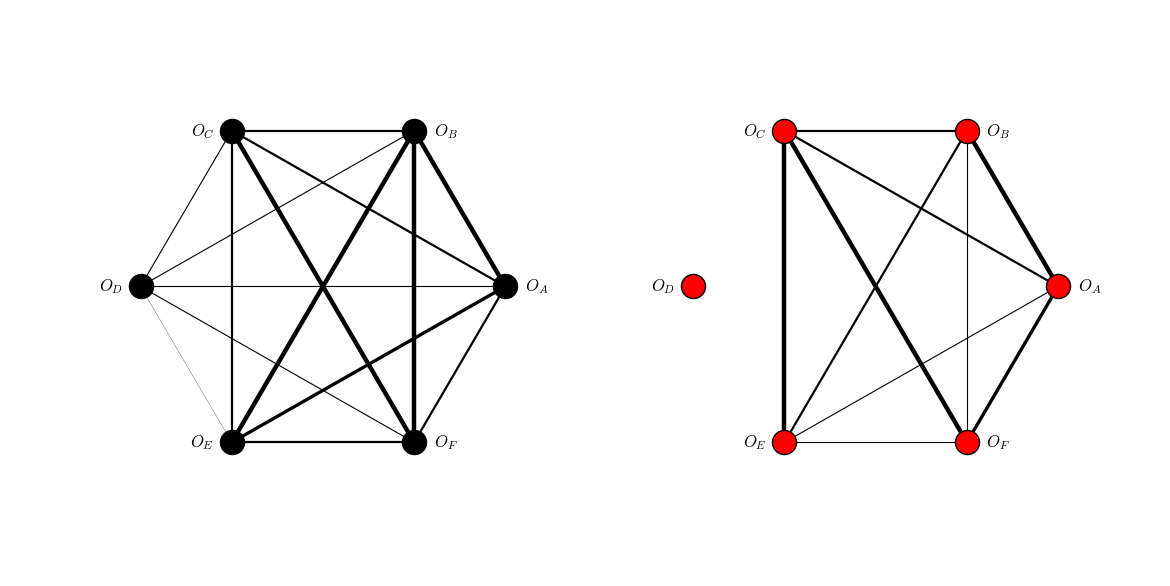
\includegraphics[scale=0.5]{figures/ramping_parameter_example.png}
	\caption[Graph representation of stylized portfolio with six obligors]{
Stylized portfolio with six obligors (A, B, C, D, E, and F).
The relative strength of the inter-obligor connections $\rho_{ij}$ is illustrated by the line-width.
In the left figure, the interdependency between customer $D$ and the other customers is rather small.
Additional to the individual inter-customer correlation each customer also has an individual obligation (symbolized by the differently coloured circles), indicated as $O_i$, $i \in \{A, B, C, D, E, F \}$.
Both the obligation of the individual customer $O_i$ and the inter-customer correlations $\rho_{ij}$ are required to compute the Concentration Risk as suggested by our measure.
For a particular value of the correlation strength obligor $D$ becomes independent from all other obligors of the portfolio.
	}
	\label{fig:6_pf_ramping}
\end{figure}

 


% \todo{add example}

% section ramping_parameter (end)


\section{Random graph models} % (fold)
\label{sec:random_graph_models}

Random graph models are widely used to understand the properties of real world networks~\cite{newman2002random}.
They provide a means of generating and analysing networks with statistical properties that resemble those of real-world networks.
The most popular random graph model is credited to %Paul Erd\"os and Alfr\'ed R\'enyi
~\cite{erdos1959random}.
One reason for its popularity is the fact that it is very simple (and analytically tractable).
Although its properties do not necessarily resemble those observed in social, financial or technical ecosystems, its dynamics already capture a very interesting phenomenon that is also relevant for this thesis: the emergence of a so-called giant component.

A connected component is a set of nodes, between which there is always a connecting path.
The giant component is a connected component for which the fraction of nodes it contains remains constant as the network grows in size.
It is also the largest component in the graph, and can be usually seen in many real world networks~\footnote{For example, in the case of the internet network, the existence of a giant component is extremely important, as it guarantees that as much nodes (computers) as possible can communicate with each otgher}.
Not only its existence is of interest, but the emergence of the giant component is an important phenomenon.
It emerges almost spontaneously as the edge density reaches a critical value, leading to a phase transition, as explained by~\cite{newman2002random}.
This can also be seen in Figure~\vref{fig:giant_component}
\begin{figure}[tb]
	\centering
	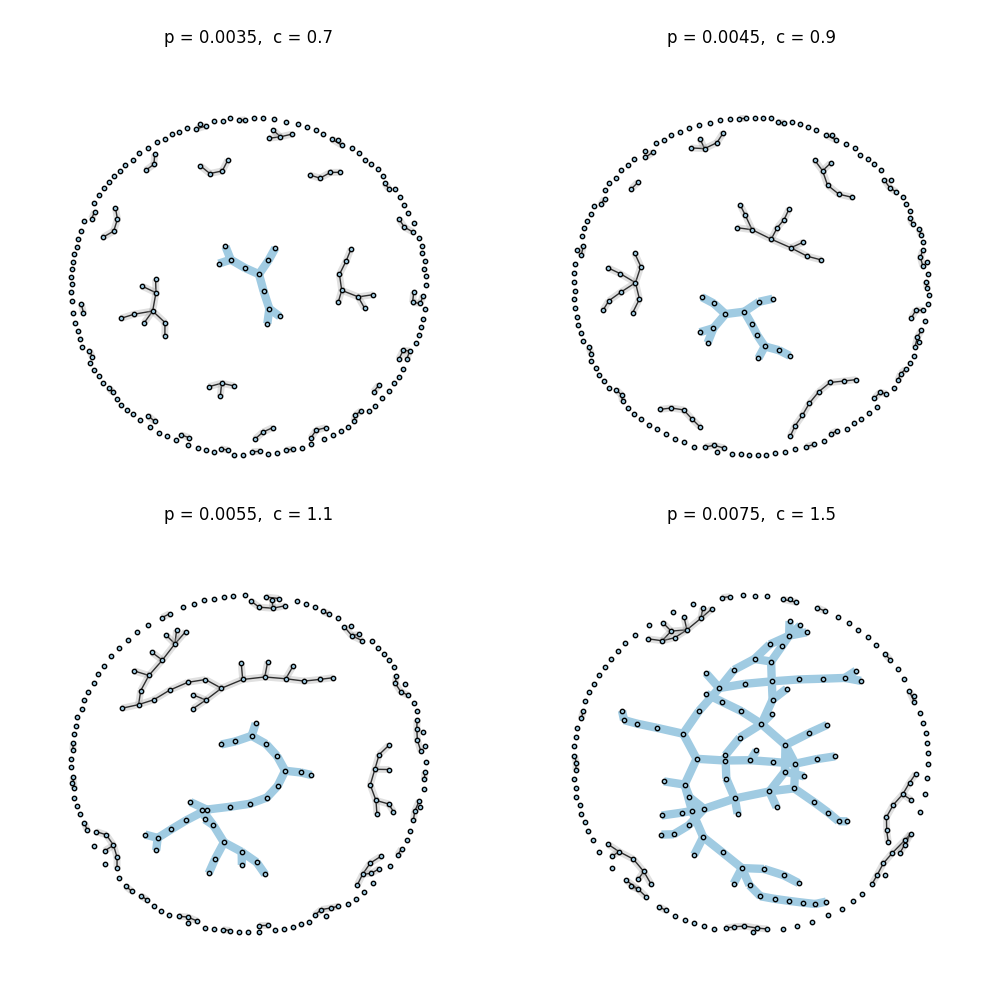
\includegraphics[width=13.5cm]{figures/giant_component.png}
	\caption[Sudden appearance of the giant component in a random graph]{This figure illustrates the sudden appearance of a giant connected component (lower plots) in the random graph model. The graphs, each with $n=200$ nodes are generated randomly, with a mean degree of $c$ and an edge probability $p$. The random graph model predicts a giant component when $c\ge1$}
	\label{fig:giant_component}
\end{figure}

One important property where the random graph model does not mimic the real world networks is the distribution of a node's degree.
The degree is a property of the node in a graph that describes how many connections (or how important these connections are) the node has to the other nodes in the graph.
Real-world networks tend to have heavy tailed distributions, where as the random graph model has a binomial distribution / Poisson distribution.
One of the these heavy tail distributions is the power law distribution, which is scale-free, as was and was shown by~\cite{Albert:2002p4071} to lead to the so-called small world phenomenon~\cite{Watts:1998db}.


% A second way in which random graphs differ from their real-world counterparts is in their degree distributions, a point which has been emphasized particularly in the work of Albert, Baraba ́si, and collaborators (Albert et al., 1999; Baraba ́si and Albert, 1999). The probability pk that a vertex in an Erd ̋os–R ́enyi random graph has degree exactly k is given by the binomial distribution:


% section random_graph_models (end)

\section{Organisation of this document} % (fold)
\label{sec:organisation_of_this_document}

This document is organized as follows.
Chapter~\ref{cha:graphs_and_networks} describes the fundamental concepts of graph theory and of the random graph model.
The random graph model provides a statistical description of the degree distribution and the component structure of random graphs, which may include both a giant component and a set of small components.
The component structure is of high relevance for providing a connection to the ramping parameter model described in Section~\ref{sec:ramping_parameter}.

In chapter~\ref{cha:ramping_parameter_under_the_random_graph_model}, we described expected properties of the ramping parameter in the case of random graphs.
This connection, based on the expected component structure, provides useful information to better understand the behaviour of the ramping parameter model for the estimation of credit concentration risk in real-world portfolios.

We finalize in chapter~\ref{cha:discussion} by providing a summary of the results of this thesis and a discussion of possible continuations of this work.
Software code used throughout this thesis is provided in the appendix.

% section organisation_of_this_document (end)

% section concentration_risk (end)

\chapter{Graphs and networks} % (fold)
\label{cha:graphs_and_networks}



The networks studied in this document can be represented by a single graph.
In general, the term \textit{graph} is used for the mathematical object defined below and the term \textit{network} for some model that relies on one (or more) graphs.

We begin by defining some terminology and proceed to described models of random graphs.

\section{Terminology and essential results} % (fold)
\label{sec:definitions_and_essential_results}

\begin{definition}A graph $G$ is a tuple
\begin{equation}
G = (V,E),
\end{equation}
\noindent where $V$ is the set of vertices (or nodes), and $E$ is the set of edges (or links).
Each edge connects exactly one pair of vertices, and a vertex-pair can be connected by maximally one edge, i.e., multi-connections are not allowed.
Let furthermore $n$ denote the number of vertices $n = |V|$ and $L$ the number of edges $L = |E|$.
\end{definition}


In this thesis, the set $V$ will correspond to the set of obligors in a portfolio, and $E$ to the interdependencies between the obligors.
In the case of a social network, for example, $V$ would be the set of persons and $E$ could mean that two persons (nodes) are acquainted (connected) with each other.

\begin{definition}A weighted graph $G$ is a graph where a number $x \in \R$ can be assigned to an element of $E$.\end{definition}

\begin{definition}An unweighted graph $G$ is a graph where no number is assigned to an element of $E$.\end{definition}


\begin{definition}The adjacency matrix $A$ of a graph $G = (V,E)$ is a matrix of size $n\times n$, such that each element $a_{ij}$ of the matrix is given by
\begin{equation}
	a_{ij} = \begin{cases}
	1 & \text{if there is an edge between $i$ and $j$, i.e. } } \{i,j\} \in E\\
	0 & \text{otherwise}
	         \end{cases}
\end{equation}
If $G$ is a weighted graph, then the 
\begin{equation}
	a_{ij} = \begin{cases}
	w_{ij} & \text{if there is an edge between $i$ and $j$ with weight $w_{ij}$ } }\\
	0 & \text{otherwise}
	         \end{cases}
\end{equation}
\end{definition}

\begin{remark}Throughout this document we will be concerned with graphs without self-edges, so that $\forall i, \, a_{ii} = 0$.\end{remark}

\begin{definition}An undirected graph $G$ is a graph where its adjacency matrix $A$ is symmetric, i.e. $\forall i,j, \, a_{ij} = a_{ji}$.\end{definition}

\begin{definition}A connected component (or just component) of an undirected graph $G = (V,E)$ is a subgraph $G' = (V', E')$ where:
\begin{enumerate}[(i)]
	\item $V'$ and $E'$ are subsets of $V$, $E$ respectively
	\item any two vertices $a,b in V'$ are connected to each other by a sequence of edges $[ e_1,\ldots, e_k]$ such that $e_1, \ldots, e_k \in E'$
	\item given a vertex $a \in V'$, for all vertices $b$ such that ${a,b} \in V'$, $b \in E'$.
\end{enumerate}\end{definition}

\begin{definition}The degree $k_i$ of a node $i$ in an undirected graph $G$ is the sum of the  elements of the $i^{th}$ row (column) of its adjacency matrix $A$, i.e. $k_i = \sum_{j=1}^{j=n} a_{ij}$ .\end{definition}
\begin{remark}In case $G$ is unweighted, then the degree of node $i$ is equal to the number of edges that connect to that node. In case $G$ is weighted, then it corresponds to the sum of the weights of the edges that connect to that node.\end{remark}


\begin{definition}The degree matrix $D$ is a graph $G$ is an $n\times n $ matrix where its diagonal contains the degree of the corresponding vertices, i.e. where $$d_{ij} = \begin{cases}
    k_i & \text{if } i = j \\
	0 & \text{ otherwise.} 
\end{cases}$$
\end{definition}

\begin{definition}The Laplacian~\footnote{Please note that there may be similar alternative definitions of the Laplacian matrix of a graph, but its properties equivalent w.r.t. the requirements for this thesis.}  matrix $L$ of a graph $G$ is given by $L = D - A$, where $D$ is the degree matrix and $A$ the adjacency matrix, as defined above.
\end{definition}

\begin{remark}The graph Laplacian turns up in a large variety of places in network modelling, including diffusion processes, random walks, graph partitioning and, the most important for the purpose of this thesis, network connectivity.\end{remark}

There is, in fact, a connection between the eigenvectors of the Laplacian matrix of a graph and its connected components, which will allow us to easily compute the component structure of particular instances of graphs.
In fact, a graph $G$ with multiple connected components $C_k$ will have a Laplacian matrix $L$ that is a block diagonal matrix.
After reordering of the vertices, each block in this matrix will be the corresponding Laplacian matrix for each component $C_k$.
\begin{theorem}
Consider a graph $G$, with a Laplacian matrix $L$. Then,
\begin{enumerate}[(i)]
	\item all eigenvalues of $L$ ${\displaystyle \lambda _{0}\leq \lambda _{1}\leq \cdots \leq \lambda _{n-1}} \lambda_0 \le \lambda_1 \le \cdots \le \lambda_{n-1}$ are $\ge 0$
	\item $\lambda_j = 0 \iff $ the corresponding eigenvector defines a connected component.
\end{enumerate}
\end{theorem}
\begin{proof}The proof is left here undone, as it can be found in most books on networks, e.g.~\cite{newman2010networks}.\end{proof}
\begin{remark}

In order to find the connected components of a graph, one can compute the null-eigenvalues and eigenvectors of its Laplacian matrix.

\end{remark}
\begin{example}{\noindent Example: }We consider the following example of a graph
\end{example}
\begin{figure}[hb]
	\centering
	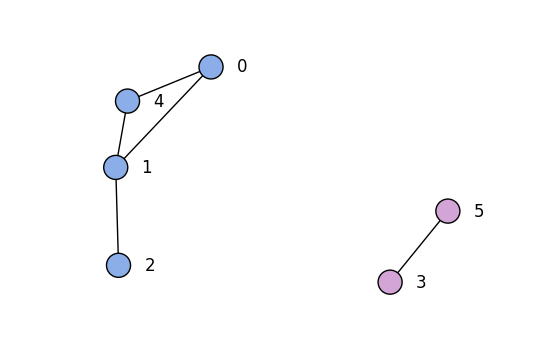
\includegraphics[scale=0.8]{figures/2_example_graph.png}
	\caption{Example graph with 2 components and 6 nodes.}
	\label{fig:example_graph}
\end{figure}
which has following (rows and columns 4,5 permutated) adjacency matrix
$$
A = \begin{bmatrix}
  0 & 1 & 0 & 1 & 0 & 0\\
  1 & 0 & 1 & 1 & 0 & 0\\
  0 & 1 & 0 & 0 & 0 & 0\\
  1 & 1 & 0 & 0 & 0 & 0\\
  0 & 0 & 0 & 0 & 0 & 1\\
  0 & 0 & 0 & 0 & 1 & 0\\
\end{bmatrix}
$$
\noindent and Laplacian matrix
% $${\begin{pmatrix}0&1&0&0&1&0\\1&0&1&0&1&0\\0&1&0&1&0&0\\0&0&1&0&1&1\\1&1&0&1&0&0\\0&0&0&1&0&0\\\end{pmatrix}}$$
$$
L = \begin{bmatrix}
  2 & -1 & 0 & -1 & 0 & 0\\
  -1 & 3 & -1 & -1 & 0 & 0\\
  0 & -1 & 1 & 0 & 0 & 0\\
  -1 & -1 & 0 & 2 & 0 & 0\\
  0 & 0 & 0 & 0 & 1 & -1\\
  0 & 0 & 0 & 0 & -1 & 1\\
\end{bmatrix}
$$
The block- structure of the Laplacian matrix is well visible and easy to correspond to the community structure in the plotted graph.

% section definitions_and_essential_results (end)


\section{Random graphs} % (fold)
\label{sec:random_graph_model}

A random graph is a graph that is generated by randomly sampling from a collection of graphs, i.e. a random variable defined in a probability space with a probability distribution.
\begin{definition}
The Erd\"os-R\'enyi random graph $G_{n, p}$ is the random graph containing $n$ nodes obtained by connecting pairs of vertices with an edge with probability $p$. Each edge exists independently with the same probability.
\end{definition}
Under this model, the probability of any simple graph $G$, i.e. without multiple edges or self-loops, with $n$ nodes and $m$ edges is given by
$$P(G) = p^m (1-p)^{\binom{n}{2} - m}$$


This model was studied by the Hungarian mathematicians Paul Erd\"os (1913-1996) and Alfr\'ed R\'enyi (1921-1970), and has lead to a large corpus of research on random graphs.
As with other models studied in this thesis, statements made about the model are statements made about the collection of graphs, rather than any specific instance of a graph.

\begin{figure}[tb]
	\centering
	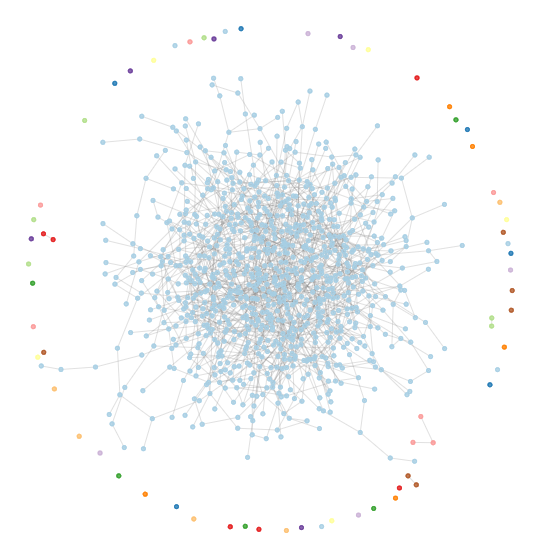
\includegraphics[width=10cm]{figures/gnp_hairball.png}
	\caption{Plot of a random graph with $n = 1000$ nodes, edge probability $p = 0.003$ and $c=3$. 
	Nodes belonging to the same connected component are coloured identically.
	We can see a dominating large component in the graph through the light blue nodes in the centre.
	The existence of this dominating component is described in section~\ref{sub:giant_component}.}
	\label{fig:hairball}
\end{figure}

The random graph model is especially interesting because several of its statistical properties can be derived analytically.
The properties of the networks it generates, however, differ substantially from those observed in real world networks~\cite{Albert:2002p4071}.

\subsection{Mean degree and degree distribution} % (fold)
\label{ssub:mean_degree_and_degree_distribution}

In the random graph model, the existence of any edge is independent from each other and solely determined by the same probability value $p$.
As such, the probability of a graph with $m$ edges drawn from the $G(n,p)$ model is given by a binomial distribution choosing $m$ edges out of a universe of $\binom{n}{2}$ edges
\begin{equation}
	P(m) = \binom{\binom{n}{2}}{m} p^m (1-p)^{\binom{n}{2}-m}
\end{equation}
Therefore, the expected number of edges is given by
\begin{equation}
	\mean{m} = \sum^{\binom{n}{2}}_{m=0} m P(m) = \binom{n}{2} p
\end{equation}
% In the course of this document, we will be not only interested on the properties of the graph itself, but also on how they build from the individual properties of the edges and nodes.
Using this result, we can derive the expected mean node degree $c$ in a graph
\begin{equation}
	c = \sum^{\binom{n}{2}}_{m=0} \frac{2m}{n} P(m) = \frac{2}{n} \binom{n}{2} p = (n-1) p,
\end{equation}

More generally, we can not only derive the mean, but also the entire distribution of the node degree.
In fact, any node in the graph is connected with independent probability $p$ to any of the remaining $n-1$ nodes in the graph.
Hence, the probability of having a particular degree $k$, i.e. being connected to exactly $k$ other nodes, is $p^k (1-p)^{n-1-k}$.
Given that there are $\binom{n-1}{k}$ possible sets of $k$ vertices, the probability distribution of the node degree is given by
\begin{equation}
    \label{eq:degree_dist_naive}
	p_k = \binom{n-1}{k} p^k (1-p)^{n-1-k}
\end{equation}


We sometimes wish to consider not only small but also large networks.
When $n$ is assumed to be large, some useful approximations can be made, which render the model more analytically tractable.

When $n\rightarrow \infty$, we can rewrite
\begin{align}
	ln[(1-p)^{n-1-k}] &= (n-1-k) \ln\left( 1-\frac{c}{n-1} \right)\\
                      &\simeq (n-1-k) \frac{c}{n-1}\\
                      &\simeq -c,\\
\intertext{\noindent and therefore }
    (1-p) ^{n-1-k} & \simeq e^{-c}
\end{align}
\noindent by using the Taylor expansion of $\ln\left(1-\frac{c}{n-1}\right)$ and approximating to the first term.
These approximations hold exactly when $n\rightarrow \infty$, as does the following approximation when
\begin{align}
    \binom{n-1}{k} = \frac{(n-1)!}{(n-1-k)! k!} \simeq \frac{(n-1)^k}{k!}
\end{align}
By applying both approximations under the assumption that $n \rightarrow \infty$, we can rewrite equation~\vref{eq:degree_dist_naive} as follows
\begin{equation}
	p_k = \frac{(n-1)^k}{k!} p^k e^{-c} = e^{-c} \frac{c^k}{k!}
\end{equation}
which is the familiar Poisson distribution.

% subsection mean_degree_and_degree_distribution (end)Mean degree and degree distribution


\subsection{Giant component} % (fold)
\label{sub:giant_component}

Although very simple, the random graph model possesses one very interesting property: the sudden appearance of the so-called giant component by varying the mean degree $c$.
A giant component is a component whose size is proportional to the size of the network $n$, and its sudden appearance is called a \textit{phase transition}.

Consider the random graph $G_{n, p}$ with two extreme parametrisations:
\begin{itemize}
	\item[] $p = 0$, there are no edges in the graph, and therefore the largest component is of size $1$,
	\item[] $p = 1$ every vertex is connected with every other vertex, and so the largest connected component has size $n$. 
\end{itemize}
Under $p=1$, the size of the largest component grows with the network.
This is called a giant component, and its size can be computed exactly in the limit of a large network size.

\begin{definition}
Let $u$ denote the average fraction of vertices not in the giant component. Let $S$ be the reciprocal of $u$, $S = 1 - u$, i.e. the average relative size of the giant component.
\end{definition}
\noindent By definition the giant component exists if and only if $u<1$. Suppose that, under the $G(n,p)$, vertex $i$ does not belong to the giant component.
Consider another vertex $j$.
Either
\begin{enumerate}[i)]
	\item $i$ and $j$ are not connected with probability $1-p$, or
	\item there is an edge between $i$ and $j$ and $j$ also does not belong to the giant component, which has a probability of $pu$.
\end{enumerate}
As such, the probability that there is an edge $(i,j)$ is $1-p + pu$.
If we now consider every node in the graph, then the probability that node $i$ is not in the giant component is $u$, and depends on it only being connected to nodes not being in the giant component.
Since every edge in the graph exists independently, then we have
\begin{equation}
	u = (1- p + pu)^{n-1} = \left[ 1 - \frac{c}{n-1} (1-u)\right]^{n-1}
\end{equation}
If we take the logarithm of both sides, 
\begin{equation}
	\ln u = \ln\left[ 1 - \frac{c}{n-1} (1-u)\right]^{n-1} = (n-1) \ln\left( 1-\frac{c}{n-1} (1-u)\right)
\end{equation}
When $n$ is large, $\frac{c}{n-1}$ is very small, so that we following approximation holds
\begin{equation}
	\ln\left( 1-\frac{c}{n-1} (1-u)\right) \approx - \frac{c}{n-1} (1-u)
\end{equation}
and therefore,
\begin{equation}
	\ln u \approx - c (1-u)
\end{equation}
By taking the exponential of both sides, we can write it as
\begin{equation}
	u \approx e^{-c(1-u)}
\end{equation}
Alternatively, one can consider the reciprocal of $u$, i.e. the fraction $S$ of nodes that do belong to the giant component.
\begin{equation}
    \label{eq:s_naive}
	S = 1 - e^{-cS}
\end{equation}
This equation has a trivial solution at $S = 0$, which is the only solution if $c \le 1$, i.e. there is no giant component if $c \le 1$.
For $c > 1$, there is not only the trivial solution but also another solution at $S > 0$.
\cite{newman2010networks} shows that the non-trivial solution best describes the giant component.

\noindent Although very simple, equation~\ref{eq:s_naive} has no closed-form solution.
It can be expressed through the \Lambert $W$-function~\footnote{The Lambert-W function is a set of functions representing the inverse relation of the function $f(z) = z e^{z}$ where $z$ is a complex number, i.e. {\displaystyle\, z=f^{-1}(ze^{z})=W(ze^{z})}}
\begin{equation}
S = 1 + \frac{W(-c e^{-c})}{c}
\label{eq:s_giant_component_lambert}
\end{equation}
\noindent, for which there are standardized numerical software module, e.g.~\cite{sympy}.

\begin{figure}[tb]
	\centering
	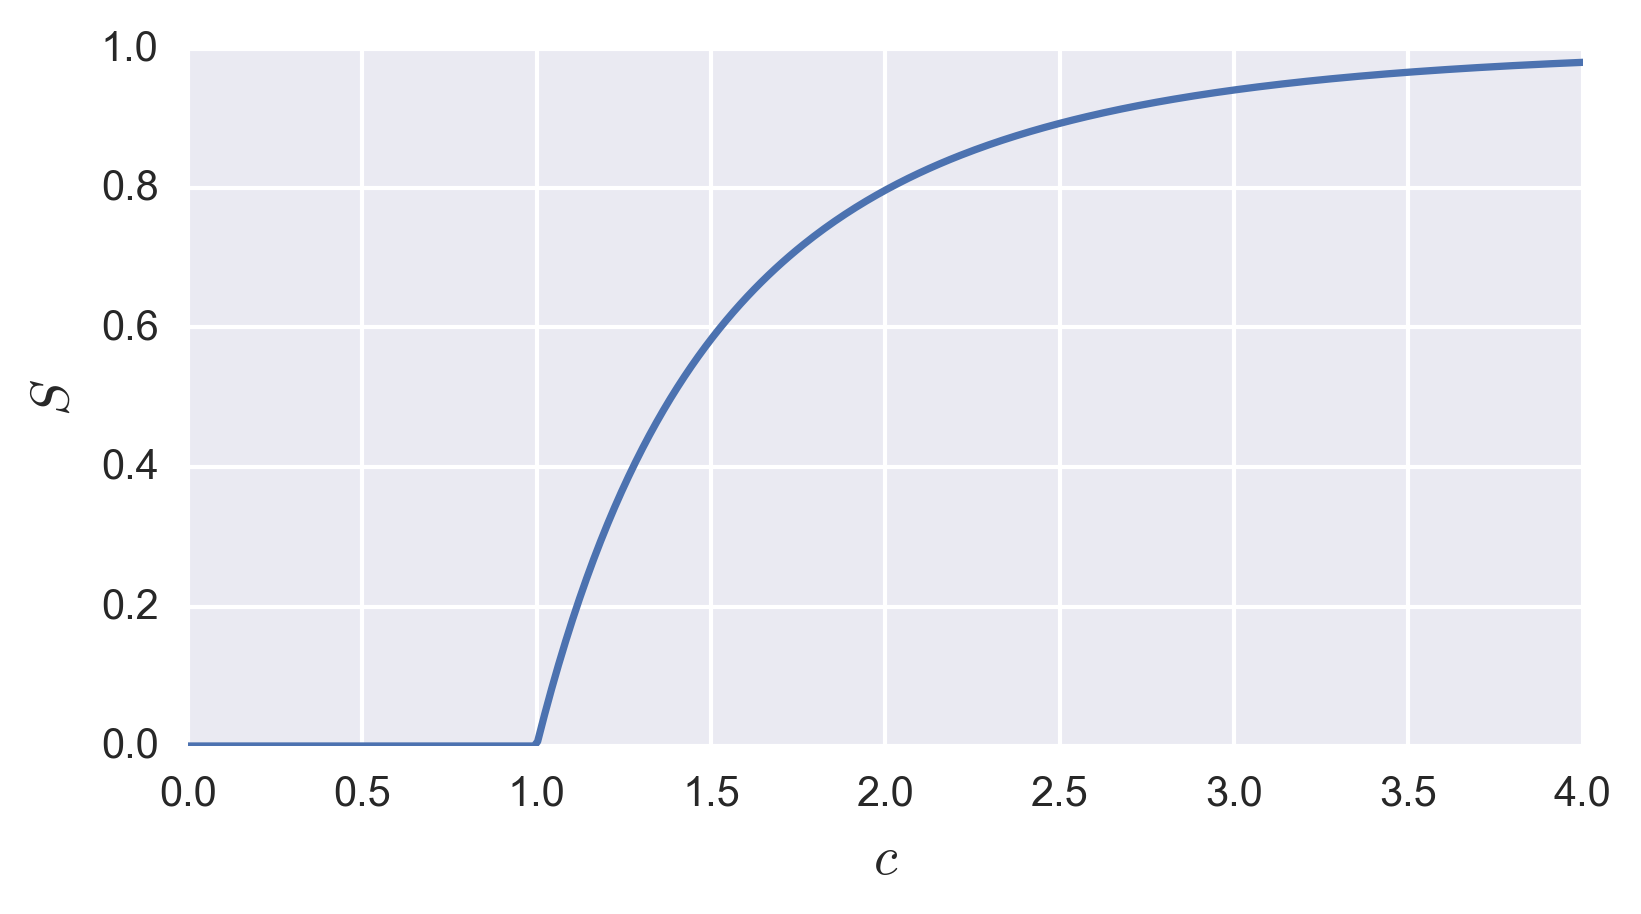
\includegraphics[]{figures/2_s_as_function_of_c.png}
	\caption{The fraction of the graph occupied by the giant component, $S$, as a function of the average expected degree $c$, and computed according to equation~\ref{eq:s_giant_component_lambert}. The phase transition at $c=1$ is well visible. For $c < 1$, no giant component is present, for $c>1$ it quickly occupies a dominating fraction of the network.}
	\label{fig:s_as_function_of_c}
\end{figure}

% subsection giant_component (end)








\subsection{Component sizes} % (fold)
\label{sub:component_sizes}


Generating functions.

The average size of $\mean{s}$ becomes 
\begin{equation}
	\mean{s} = \frac{1}{1-c-cS}
\end{equation}
with $S$ being the fractional size of the giant component, as given by equation~\ref{eq:s_giant_component_lambert}.

% subsection component_sizes (end)


% section random_graph_model (end)



\section{Generating functions} % (fold)
\label{sec:generating_functions}



We assume throughout this chapter that  follow~\cite{Newman:zFi032Kd}, which defines a set of generating functions for the probability distributions of some of the statistical properties of the graphs.
The basis of these is the function $G_0(x)$ for the probability distribution of vertex degrees $k$, defined as
\begin{equation}
G_0(x) = \sum_{k=0}^{\infty} p_k x^k
\end{equation}
where $p_k$ is the probability that a given vertex of the graph has degree $k$.

- normalization assumption ($G_0(1) = 1$)
- $G_0(x)$ is finite for all $|x| \le 1$

The derivatives of this function can be used to derive other statistical quantities.
For example, one can recover the probability $p_k$ by taking the $k^{th}$ derivative of the $G_0$
\begin{equation}
	p_k = \frac{1}{k!} \frac{d^k G_0}{dx^k} \Big|_{x=0}.
\end{equation}

Furthermore, one can obtain the average degree $z$ of the nodes in a graph 
\begin{equation}
	z = \mean{k} = \sum_k k p_k = G'_0(1)
\end{equation}

The function is given by the polylogarithm function
\begin{equation}
	\poly{n}{z} = \sum_{k=1}^{\infty} \frac{z^k}{k^n}
\end{equation}

\subsubsection{Component sizes} % (fold)
\label{ssub:component_sizes}

$H_1(x)$ follows the recursive condition
\begin{equation}
	H_1(x) = x G_1( H_1(x))
\end{equation}








\begin{equation}
\mean{s} = 1 + \frac{G'_0(1)}{1-G'_1(1)}	
\end{equation}




For a Poisson random graph







For a power law graph, this is given by
\begin{equation}
	G_1(x) = \frac{\poly{\tau-1}{xe^{-1/\kappa}}}{x\poly{\tau-1}{e^{-1/\kappa}}}
\end{equation}
and therefore
\begin{equation}
	G'_1(x) = \frac{\operatorname{Li}_{s - 2} \left(x e^{- 1/\kappa}\right)}
	               {x^{2} \operatorname{Li}_{s - 1}\left(e^{- 1/\kappa}\right)} -
	          \frac{\operatorname{Li}_{s - 1}\left(x e^{- 1/\kappa}\right)}
	               {x^{2} \operatorname{Li}_{s - 1}\left(e^{- 1/\kappa}\right)}
\end{equation}




In some networks, the degree distribution for large values is not quite a power law, while for small values it is. This is particularly appropriate when there are costs associated with having large degrees. For example, building and maintaining a large social network, or publishing papers with many people, requires time and energy, both of which are limited. Therefore, one cannot really expect to see the huge fluctuations that are predicted by power-law distributions. A related model is a power law with an exponential cut off, where the probability mass function is given by
\begin{equation}
	p_k = ck^{-\tau} e^{− k / A}, k \ge 1,
\end{equation}

for some large A. Thus, for k small compared to A the distribution looks like a power law, while for values that are large compared to A the exponential decay takes over.
We continue to discuss the notion of highly connected graph sequences.


% subsubsection component_sizes (end)Component sizes
% section generating_functions (end)



\section{Configuration model} % (fold)
\label{sec:configuration_model}

The configuration model is one of the most popular null models for the study of the statistical properties of networks.
It is inspired 

% section configuration_model (end){Configuration model}


% chapter graphs_and_networks (end)
\chapter{Ramping parameter under the random graph model} % (fold)
\label{cha:ramping_parameter_under_the_random_graph_model}

Previous work~\cite{Sindel:2009vd} provided a connection between the clustered structure of a graph and an interpretation of concentration risk.
The methodology presented by the authors considered the effects of removing edges with weight under given a varying threshold on the community structure of a fully connected obligor-correlation matrix.
In particular, by computing the variation of the component structure of the graph, the authors have shown how to analyse concrete credit portfolios and identify sets of highly connect assets.


This thesis builds upon the aforementioned model and aims at describing the expected behaviour of the ramping parameter model for theoretical graph generation models.
In this chapter, we focus on the random graph model, a well understood theoretical graph model, described in section~\vref{sec:random_graph_model}.

In particular, it tries to describe the expected behaviour of the curve designed by the~\cite{Sindel:2009vd} the problem from the perspective of having
large, idealized portfolios 
and a random graph model that generates them.





\section{The ramping parameter model} % (fold)
\label{sec:the_ramping_parameter_model}


The approach proposed by~\cite{Sindel:2009vd} for quantifying the concentration risk of a loan portfolio works can be summarized as follows:
\begin{itemize}
	\item The mutual dependency between the obligors in a portfolio is represented by a matrix $\rho_{ij}$. This matrix is symmetric, the values $\rho_{ij} \in [0,1]$, and it will be called correlation matrix throughout the remainder of this document.
	\item A so-called ramping parameter $\ramp \in [0,1]$ is used to define the effective correlation matrix $\rho_{ij}(\ramp)$ given the value of this  parameter:
	\begin{equation}
	\rho_{ij}(\ramp) = 
		\begin{cases}
		1 \text{ if } \rho_{ij} \ge \ramp,\\
		0 \text{ otherwise}.
		\end{cases}
	\end{equation}
	At $\ramp = 0$, the effective matrix will contain all connections in the original matrix. At $\ramp = 1$, all obligors in the effective matrix will be disconnected.
	
	\item The exposure-dependence is taken into account by computing the “effective” exposure for every value of $\ramp$.
\end{itemize}

To properly account for the Concentration Risk we compute the ratio $R(ρ∗)$ of the maximum of all exposures of all identified connected components $C_k$ and the total exposure of the portfolio
of the portfolio and $j$ runs over all loans within the connected component $C_k$.
\begin{figure}[tb]
	\centering
	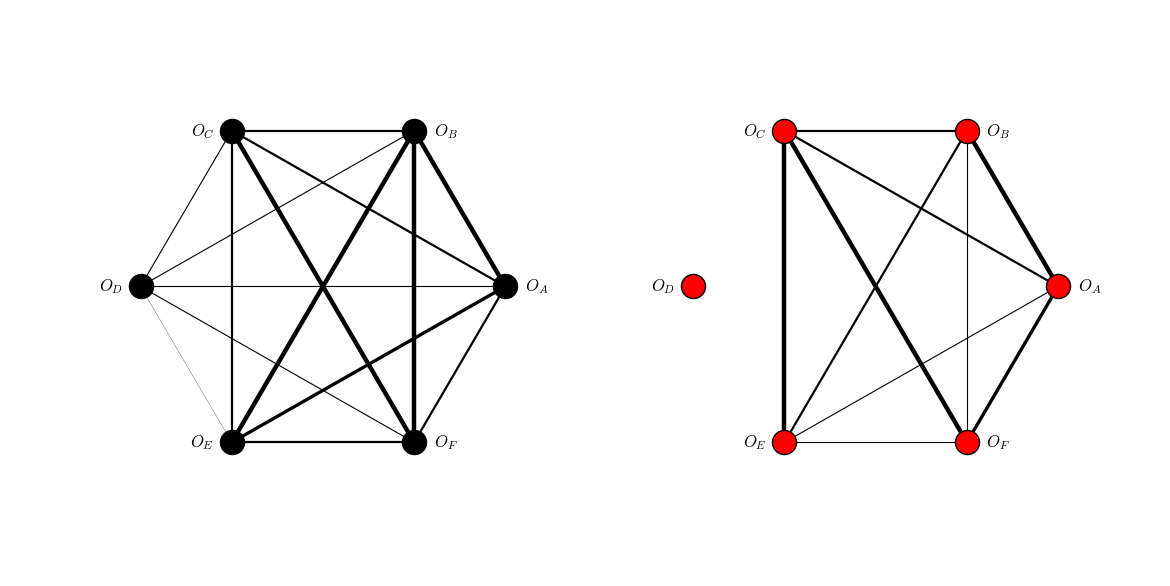
\includegraphics[scale=0.5]{figures/ramping_parameter_example.png}
	\caption{
Stylized portfolio of six obligors (A, B, C, D, E, and F).
The relative strength of the inter-obligor connections $\rho_{ij}$ is illustrated by the line-width.
In the left figure, the interdependency between customer $D$ and the other customers is rather small.
Additional to the individual inter-customer correlation each customer also has an individual obligation (symbolized by the differently coloured circles), indicated as $O_i$, $i \in \{A, B, C, D, E, F \}$.
Both the obligation of the individual customer $O_i$ and the inter-customer correlations $\rho_{ij}$ are required to compute the Concentration Risk as suggested by our measure.
For a particular value of the correlation strength obligor $D$ becomes independent from all other obligors of the portfolio.
	}
	\label{fig:6_pf_ramping}
\end{figure}

 
 
% And the next is a somewhat informal definition
 
\begin{definition}{Portfolio}
A credit portfolio is a tuple $(O, \hat{\rho})$, where $O$ is a set of $n$ exposures from $n$ different obligors and $\hat{\rho}$ an $n \times n$ matrix.
The $\rmat$ matrix represents the interdependency (or correlation) between each obligor $i$, and each element $\rij \in [0,1]$.
\end{definition}

\begin{remark}
Throughout this work, the matrix $\rmat$ is symmetric, so that $\forall i,j \rij = \rho_{ji}$ and the values of $\rho_{ij}$ are positive.
Even though in the real world the dependency between obligors is not necessarily symmetric, e.g. in the case where obligor $i$ is asubsidiary of obligor $j$, the symmetry assumption renders the model more analytically tractable.
\end{remark}



The algorithm is described in~\ref{algo:ramping_parameter}.

\begin{algorithm}
\label{algo:ramping}
\caption{Ramping parameter algorithm~\label{algo:ramping_parameter}}
\State $\ramp \gets 0$

\State $w$ \gets \textrm{order $O_{ij}$}

\State $C$ \gets \{\}

\State $\epsilon\gets \min\{w_{ij}\}$

% 1. We systematically increase the ramping parameter ρ∗ from 0 to 1 with a suffi- ciently small step size.
\For{$\ramp$ \in [0,1]}

	M \gets \text{compute the obligor correlation matrix as shown in eq~\ref{}

	G \gets ({O, {m_{ij}})

	C \gets \text{all connected connected components of graph} G

	R(\ramp) \gets \max_{C_k} \left(  \frac{\sum_{j\in C_k} \textrm{EAD}_j}{\sum_i \textrm{EAD}_i}  \right), where C_k\\

\EndFor
\end{algorithm}

% 2. For each value of ρ∗ we compute the effective (inter) obligor-correlation matrix as shown in Eq. 3.2.
% 3. We compute the number of connected components and the corresponding obli- gation in each component of the graph for every value of ρ∗.4
% 4. To properly account for the Concentration Risk we compute the ratio R(ρ∗) of the maximum of all exposures of all identified connected components Ck and the total exposure of the portfolio
% of the portfolio and j runs over all loans within the connected component Ck.

% In Eq. (3.3) i runs over all loans of the portfolio, i EADi is the total obligation
% Note that R(ρ∗) describes the risk of a portfolio associated with the default of its biggest clump for a given ρ∗. The risk related to a correlated default of the two biggest clumps - which has a very small probability - is not included in equation (3.3). Of course one could account for such scenarios in R(ρ∗) as well by adjusting formula (3.3). As correlated defaults are exponentially suppressed we do not incorporate them in


% section the_ramping_parameter_model (end)

\section{Ramping parameter under random graph model} % (fold)
\label{sec:ramping_parameter_under_random_graph_model}


In this section, we will using properties of the random graph model in order to make predictions about the ramping parameter and the concentration risk.
Contrasting to the original work on the ramping parameter~\cite{Sindel:2009vd}, rather than computing the concentration risk of a particular portfolio, we wish to see the behaviour of the family of portfolios drawn from a given distribution.
In order to do this, certain assumptions about the portfolios must be made.
In particular, we assume:
\begin{itemize}
	\item the portfolios to be large, i.e. we assume that $n \rightarrow \infty$, where $n$ is the number of obligors
	\item the exposure of each individual obligor is $\frac{1}{n}$, i.e. the exposure is uniformly distributed amongst all obligors
	\item the elements of the dependency matrix to be independent from each other
\end{itemize}

\begin{remark}The dependency to large $n$ allows the results for the random graph model to hold exactly.
In practice, however, even large portfolios will be finite and there will be some error.
\end{remark}




\begin{definition}
\label{def:equivalence_aux} 
Let $\rho \in \R$, and the function $f_\rho$ so that
\begin{equation}
\label{eqn:function}
f_\rho: C \rightarrow A\\
\\
a_{ij} = \begin{cases} 1 & \text{if } c_{ij} > \rho \\
                       0 & \text{if } c_{ij} \le \rho \\
                       0 & \text{if } i = j
        \end{cases}
\end{equation}
Let $g$ the pdf and $G$ the cdf of each element $c_{ij}$ of $C$.

By defining $p = 1-G(\rho)$, we can write
$$
P( a_{ij} = 0 ) = P(c_{ij} \le \rho) = G(\rho) = 1-p
$$
and conversely
$$
P( a_{ij} = 1 ) = P(c_{ij} > \rho) = 1 - G(\rho) = p
$$
\end{definition}

In a first step we define the space of correlation matrices 
\begin{definition}
The space of correlation matrices $\mathcal{C}_{n\times n} = \left( C, \mathcal{F},  g_C \right)$ consists of all matrices where
\begin{itemize}
\item[-] $C \in \R^{n \times n}$, such that $c_{ij} = c_{ji}$, $c_{ii} = 0$, 
\item[-] $\mathcal{F}$ is the Borel $\sigma-$algebra on $C$,
\item[-] and all elements $c_{ij}$ are i.i.d. random variables with a probability distribution $g$.
\end{itemize}
\end{definition}

We want to identify matrices in $\mathcal{C}$ with adjacency matrices using a construction like the function \ref{eqn:function} defined above.
As the image of $f$ depends only on $G(\rho)$  this map is not injective; more precisely two matrices $C_1$ and $C_2$ are mapped to the the same matrix $A$ if for each pair $i\neq j$ of indices the equation  $G(\rho) = 1-p$ is satisfied.
We use this relation to define equivalence classes:

\begin{definition}
\label{def:equiv_correlation}
Two matrices $C_1$ and $C_2$ are equivalent if the following condition is satisfied:
\begin{equation}C_1\sim C_2\quad \Leftrightarrow \quad \forall i,j \,\ f_{\rho}(c^1_{ij}) = f_{\rho}(c^2_{ij})\,.\end{equation}
Then the space of equivalence classes is denoted by $\widetilde{C}_{n\times n}$. 
\end{definition}



\begin{theorem}{Equivalence to random graph model}
\label{thm:equivalence_random_graph_model}
Consider the following probability spaces:
\begin{enumerate}
	\item the space of equivalence classes of correlation matrices $\widetilde{C}_{n\times n}$,
	\item the space of unweighted adjacency matrices $\mathcal{A}_{n\times n} = \left( A, 2^A, P_A \right)$,
	\item the space of random graphs $G_{n,p}$
\end{enumerate}
\noindent where,
\begin{itemize}
	\item[] $A \in \{0,1\}^{n \times n}$ such that $\forall i,j\,  a_{ij} = a_{ji} \text{ and } a_{ii} = 0$,
	\item[] $P_A = \begin{cases} 1 & \text{with probability } p,\\0 & \text{with probability } 1-p\end{cases}$,
	\item[] $P_C$ is some probability distribution,
	\item[] an adjacency matrix is a (0,1)-matrix with zeros on its diagonal.
\end{itemize}
The probability spaces are equivalent.
\end{theorem}

\begin{proof}

(2) $\Leftrightarrow$ (3):
Given that (i) a graph is defined unequivocally by its adjacency matrix, that (ii) all elements of $a_{ij}$ are by definition independent and that (iii) $P_A$ follows the same probability distribution as in $G_{n,p}$, both probability spaces are equivalent.
 % follows by the definition of $G_{n,p}$.
\\
(1) $\Leftrightarrow$ (2):
The equivalence of $\widetilde{\mathcal{C}}_{n\times n}$ and $\mathcal{A}_n$ is a direct consequence of the definition~\ref{def:equiv_correlation} of the equivalence classes \\
\end{proof}


\vspace{0.5cm}

By making an assumptions on the distribution of the portfolio interdependency or correlation matrix $\rmat$, theorem~\vref{thm:equivalence} allows us to apply the results of the random graph model to the study of the ramping parameter.
The original work of~\cite{Sindel:2009vd} assumes $\rhoij$ to be a non-negative correlation value in the interval $[0,1]$, and relies on the empirical distribution of the portfolio values.
% without making any expl assumptions on the distribution of the values.

In practice the matrix $\rmat$ can be generated by multiplying a set of (independent or correlated) risk factors with the dependencies of each obligor to these risk factors.
\todo{example}
Alternatively, it could also be generated either by expert knowledge (in which case one would expect the matrix to be rather sparse), by a pure correlation of stock prices of the obligors, or even by a hybrid approach.

In light of this, no general assumptions can be made over the distribution of the values of $\rmat$ and we will be studying the behaviour of the ramping parameter under the following distributions:
(1) the uniform distribution, and (2) the truncated exponential distribution.


\subsection{Giant component} % (fold)
\label{sub:giant_component}

As seen in section~\vref{sub:giant_component}, \vref{eq:s_giant_component_lambert} the giant component of the $G_{n,m}$ exists when $c \ge 1$, $c$ being the mean degree of $G$.
This means that a giant component is expected to exist when each vertex is in average connected to at least one other vertex.
As we have seen, the relative size $S$ of the giant component is given by:
\begin{equation}
	S = 1 + \frac{W(-c e^{-c})}{c},
\end{equation}
\noindent where $W$ is the Lambert-$W$ function.
Although there is no closed-form solution for this equation, it is possible to solve it numerically.

The largest connected component of the effective correlation matrix is essential to computing the ramping parameter.
Whenever it exists, the giant component is therefore relevant.

We note that, under theorem~\ref{thm:equivalence_random_graph_model}, the mean degree $c$ is connected to the distribution of the values of the correlation matrix by its c.d.f..
In fact, $c = p (n-1)$, which as we defined in~\ref{def:equivalence_aux} can be rewritten as $c = (1-G(\rho)) (n-1)$, where $G$ is the c.d.f. of the elements of the correlation matrix.


\subsubsection{Uniform distribution of obligor correlations} % (fold)
\label{ssub:uniform_distribution}

By assuming that the $\rij \sim  U(0,1)$, the c.d.f. is trivially $G(\rho) = \rho$, and therefore $c = (1 -\rho)(n-1)$.
As we will see, the giant component therefore appears at a very early stage in the evolution of the ramping parameter, and so the community structure will be largely dominated by it, which can be seen in~\vref{fig:uniform_giant_component}.
\begin{figure}[tb]
	\centering
	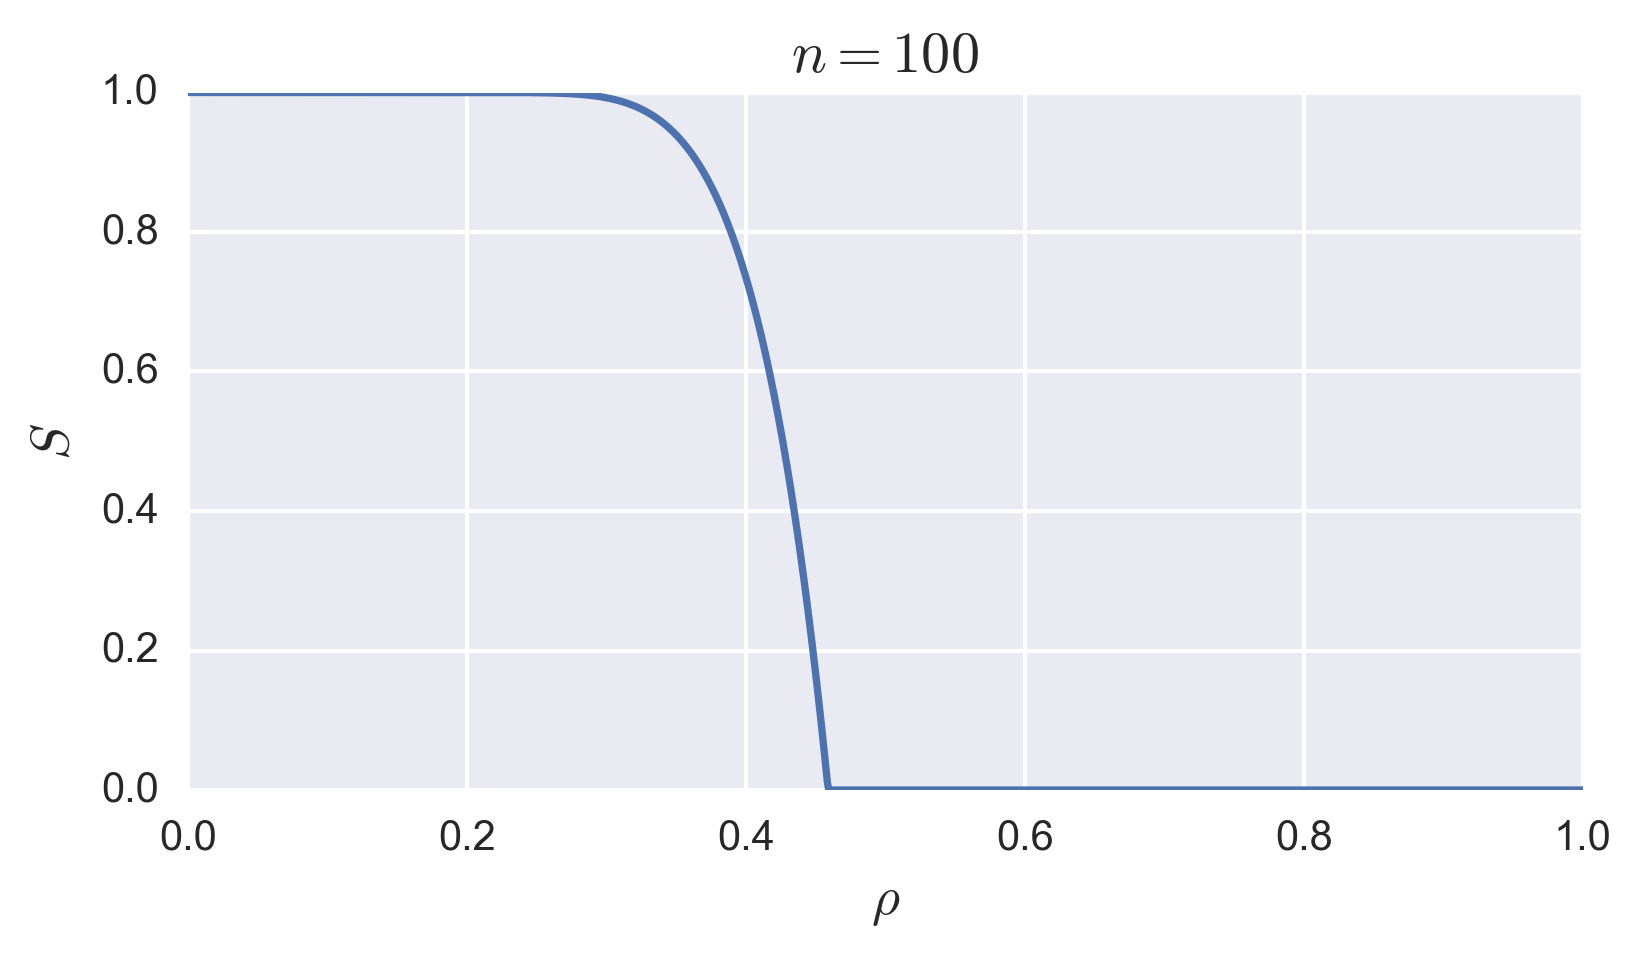
\includegraphics[scale=.8]{figures/3_uniform_giant_component.png}
	\caption{Relative size $S$ of giant component as a function of the ramping parameter $\rho$ given an uniform distribution of the correlation weights.}
	\label{fig:uniform_giant_component}
\end{figure}

% subsubsection uniform_distribution (end)

\subsubsection{Truncated exponential distribution} % (fold)
\label{ssub:truncated_exponential_distribution}

As we have seen in section~\ref{ssub:uniform_distribution}, the giant component clearly dominates the community structure of the graph for the most values of the ramping parameter.
In a real world portfolio, it is likely that most correlations will be near zero, and that the latent structure of the inter-obligor matrix is revealed by a small set of strong interconnections.

In order to represent this, we assume that the $\rij$ are distributed according to the truncated exponential distribution.
The distribution is similar to the exponential distribution, but it is restricted to the domain $[0,1]$.
Like the exponential distribution, it is governed by one parameter: $\alpha$.
Its p.d.f. is as follows
\begin{equation}
	g(x) = - \frac{\alpha e^{- \alpha x}}{1-e^{-\alpha}}
\end{equation}
\noindent and the c.d.f. given by
\begin{equation}
	G(x) = \frac{1 - e^{-\alpha x}}{1-e^{-\alpha}}.
\end{equation}
The behaviour of the p.d.f. can be seen in figure~\vref{fig:exponential_distribution}. Larger values of the parameter $\alpha$ lead to more probability being concentrated with lower values of the r.v..
\begin{figure}[tb]
	\centering
	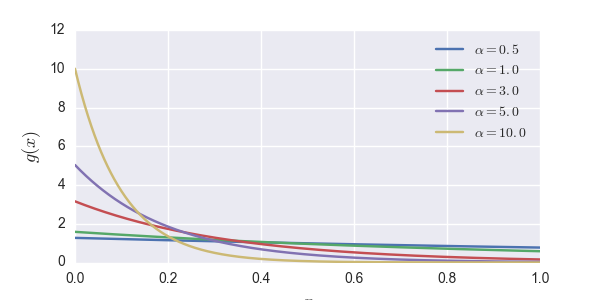
\includegraphics[scale=.8]{figures/3_exponential_distribution_pdf.png}}
	\caption{Probability density function of truncated exponential distribution with different values of the parameter $\alpha$.}
	\label{fig:exponential_distribution}
\end{figure}
The fact that much more probability density is concentrated on lower correlation values leads to an earlier and smoother disaggregation of the giant component.
The point at which the giant component disappears is also strongly dependent on the value of the parameter $\alpha$, which can be observed in figure~\vref{fig:exponential_giant_component}.
\begin{figure}[tb]
	\centering
	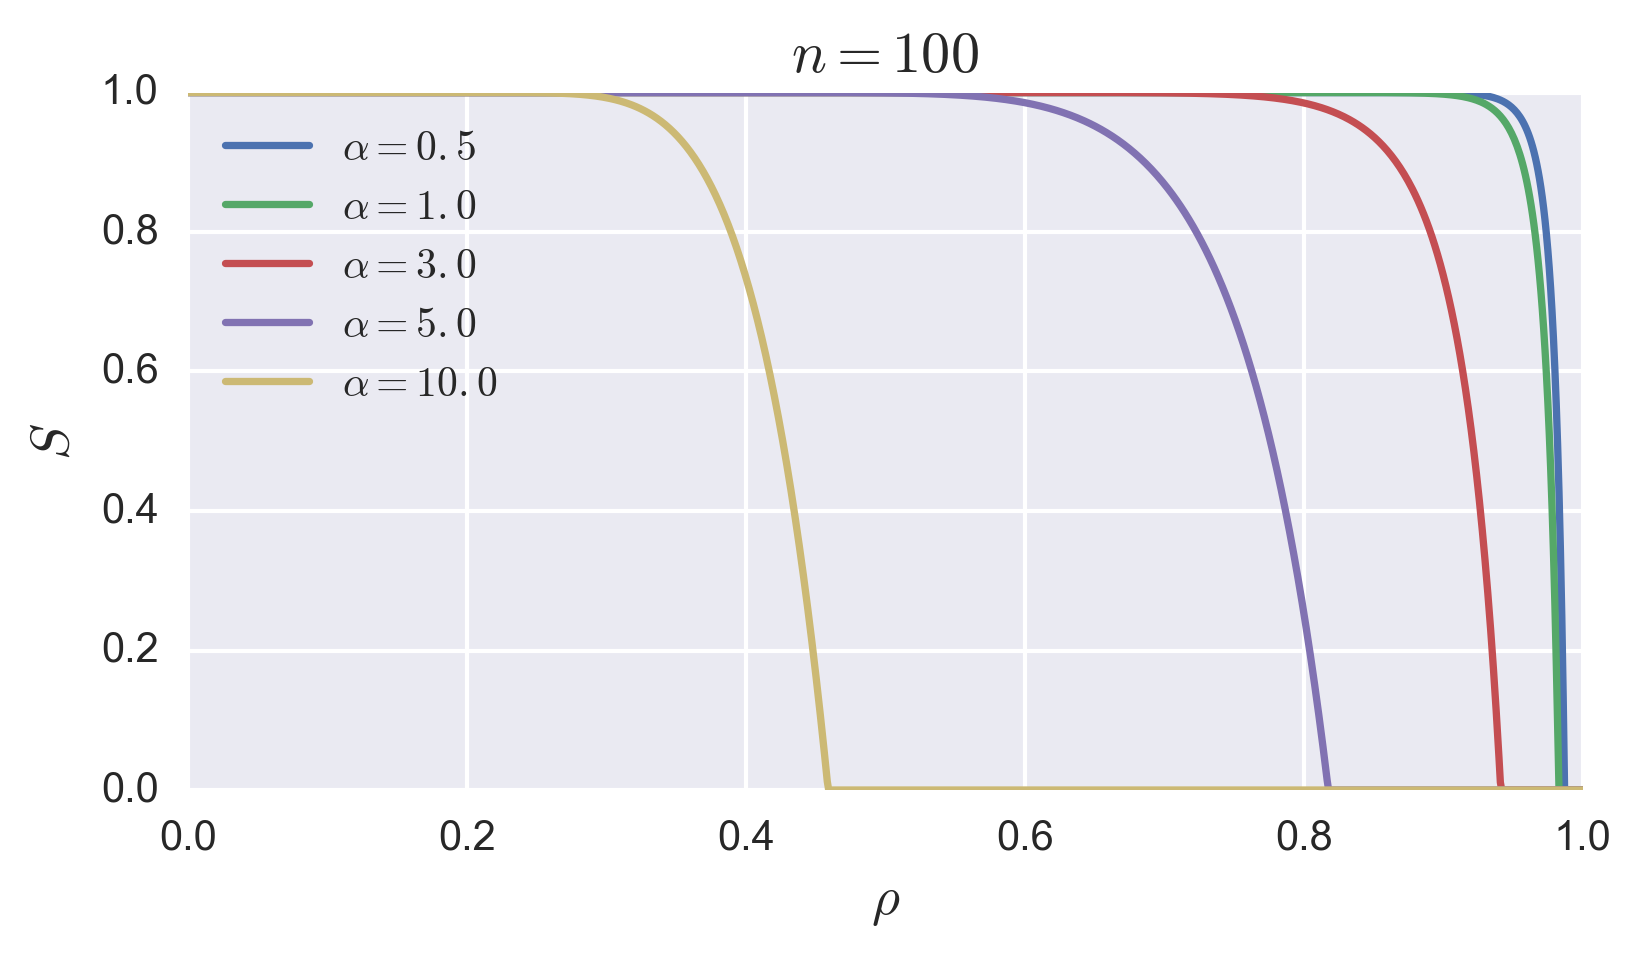
\includegraphics[scale=.8]{figures/3_exponential_giant_component.png}
	\caption{Relative size $S$ of giant component as a function of the ramping parameter $\rho$ given truncated exponential distributions  of the correlation weights with different parameters $\alpha$.}
	\label{fig:exponential_giant_component}
\end{figure}
This is already of great interest to the study of the ramping parameter, since it indicates a strong sensitivity to the distribution of the correlation values, independently of whether additional structure being available (which goes beyond of this chapter).

% subsubsection uniform_distribution (end)



% subsection giant_component (end)

\subsection{Small components' sizes} % (fold)
\label{sub:component_sizes}

% Using the random graph model we know 
From the previous chapter, we know that in the random graph model, the probability distribution of $\pi_s$, i.e. the probability that a randomly chosen node in the graph belongs to a component of size $s$.
We also know that this distribution complements the giant component
\begin{equation}
	\sum_{s=1}^{\infty} \pi_s = 1 - S
\end{equation}
\noindent and that it is given by
\begin{equation}
	\pi_s = \frac{1}{s!}\left[  \frac{d^{s-1}}{dh^{s-1}}e^{s c(h-1)}  \right] = \frac{e^{-s c} (s c)^{s-1}}{s!},
\end{equation}
What we are interested is, however, the actual number of components with size $s$.
This can be easily derived by considering that $n_s$ will be related to $\pi_s$ in that $s$ nodes will belong to a component of size $s$.
Therefore, 
\begin{equation}
	n_s = \frac{\pi_s}{s} = \frac{e^{-s c} (s c)^{s-1}}{s\,s!}.
\end{equation}
% We can see, 



% subsection component_sizes (end)





\begin{figure}[tb]
	\centering
	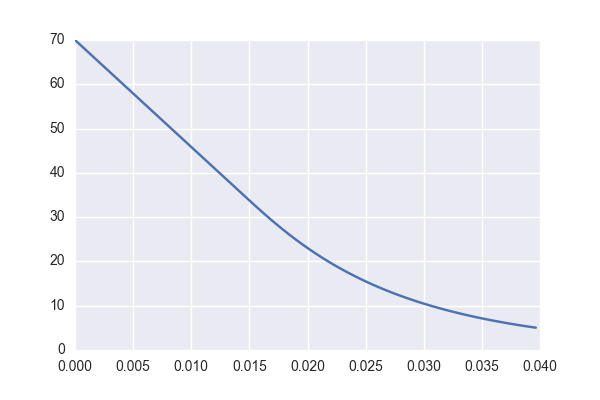
\includegraphics[]{figures/gnp_number_components.png}
	\caption{Number of components as a function of the probability $p$ of the $G(n,p)$ model.}
	\label{fig:figure1}
\end{figure}


\begin{itemize}
	\item The variation of the ramping parameter is equivalent to having random graphs generated with different $p$ probabilities.
\end{itemize}


describe the phase transition


describe the size of the components

% section ramping_parameter_under_random_graph_model (end)

% chapter ramping_parameter_under_the_random_graph_model (end)
% \chapter{Ramping parameter under the configuration model} % (fold)
\label{cha:ramping_parameter_under_the_configuration_model}

Power law functions


% chapter ramping_parameter_under_the_configuration_model (end)
\chapter{Summary and discussion} % (fold)
\label{cha:discussion}

This thesis explores properties of the ramping parameter model~\cite{Sindel:2009} for the random graph model.
To the best of our knowledge, this has not been addressed in the literature.
% In particular, the random graph model by~\cite{} and the configuration model were explored.
% The study of the theoretical properties of the ramping parameter is, to the best of our knowledge, not in the literature.



The random graph model is a simple model of network formation, which generates networks with different statistical properties than real-world networks, but from which analytic solutions can be derived.
For studying the ramping parameter model, this is an interesting model to explore, since it has very relaxed assumptions:
\begin{itemize}
\item every edge exists independently from each other
\item the properties of the edges are unclear
\end{itemize}

% The configuration model generates networks that follow an input degree distribution.
% This is an important property, since degree distributions of real-world networks have properties that are independent of the domain of the network.
% For example....



state the assumptions of the thesis

state the results


\section{Future work}
\label{sec:future_work}

What is the most adequate model for studying obligor interdependency?
Are the power law graphs the best?
Is there a correlation between the weight and the degree of the weight matrix?


Configuration model
effect of edge removal from power-law and power-law like degree distributions~\cite{dubois2012effect}





Directed graphs.
There is a treatment of the directed graphs model with the generating functions.
Theoretical properties of connectedness are, however, cannot easily be derived from them.



Connection to the study of real portfolios.
How to use the studied properties as null models for the ramping parameters of real networks?
Is there a connection to other measures of the concentration risk?


The ramping parameter its concern with the study of a measure for concentration risk.
In a risk management Setting, it would also be important to be able identify the obligors that increase the risk portfolio, or even of providing information regarding new credits / obligors that can be added to the portfolio so that the concentration risk effectively diminishes.


% section future_work (end)

% chapter discussion (end)

%now enable appendix numbering format and include any appendices
\appendix
\chapter{}
\section{Python code}


% 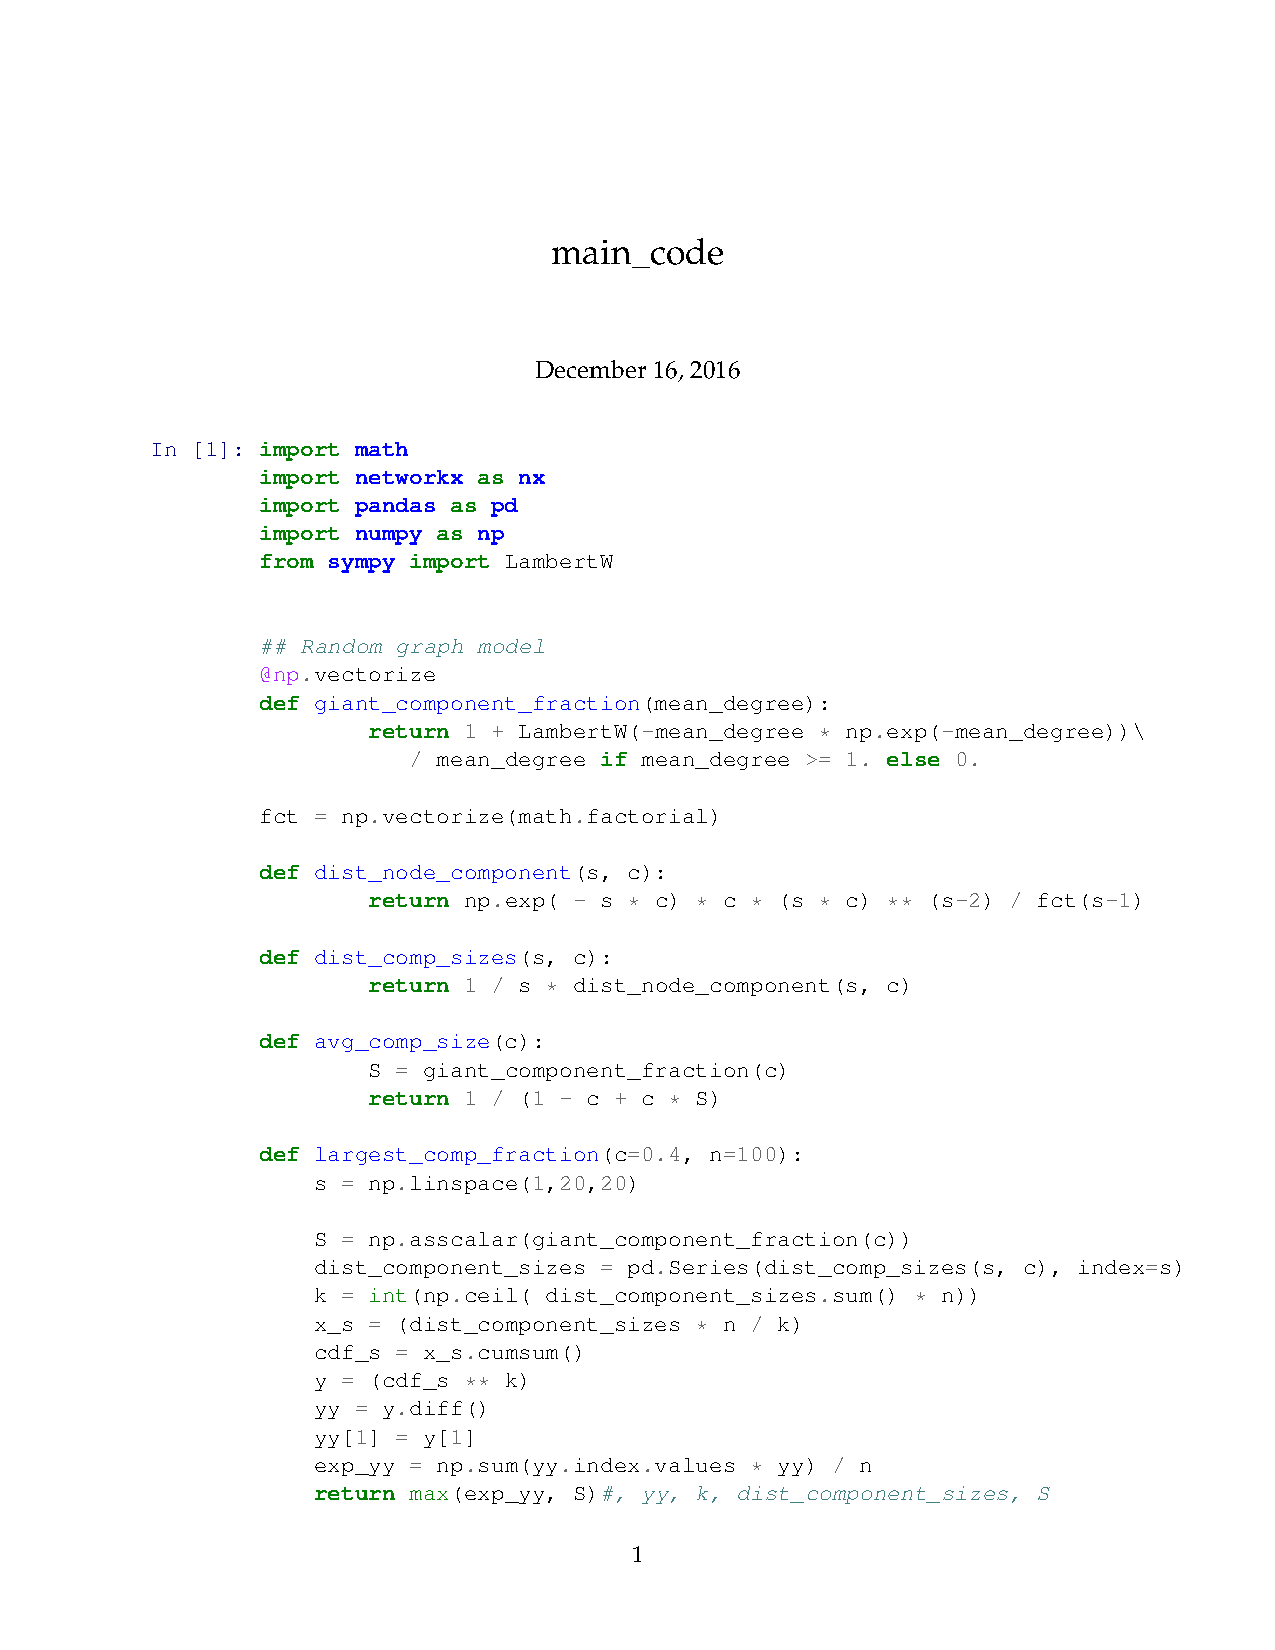
\includepdf[pages={1-2}]{main_code.pdf}

\setboolean{@twoside}{false}


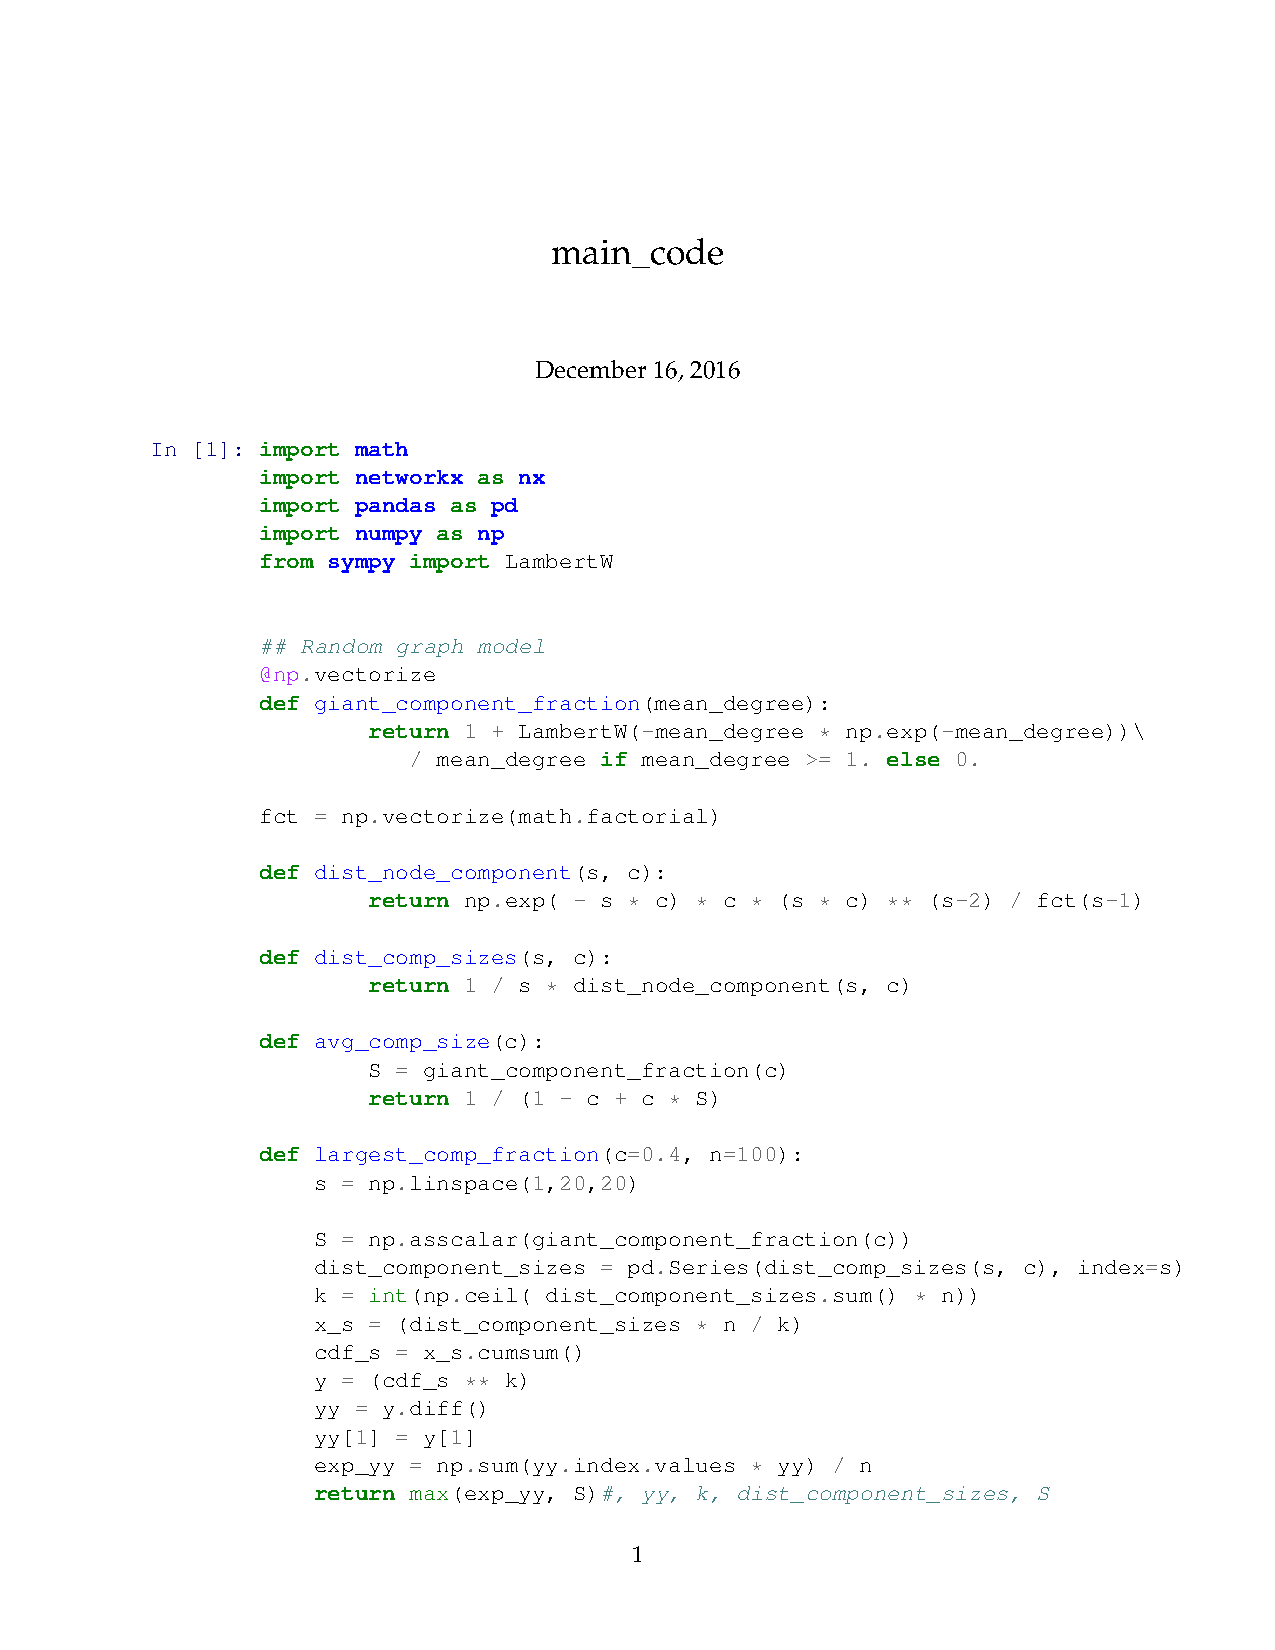
\includepdf[pages=-]{main_code.pdf}
% \include{appendix2}

%next line adds the Bibliography to the contents page
\addcontentsline{toc}{chapter}{Bibliography}
%uncomment next line to change bibliography name to references
\renewcommand{\bibname}{References}
\bibliographystyle{apalike}  %use the plain bibliography style
\bibliography{bibliography/biblio}        % use a bibtex bibliography file refs.bib


\end{document}

